\documentclass[a4paper,12pt]{article}
\usepackage[left=2cm,right=2cm,top=2cm,bottom=2cm]{geometry} % Do ustawień marginesów
\usepackage{multicol} % Dla podziału na kolumny
\usepackage{ragged2e} % Dla justowania tekstu
\usepackage{graphicx} % Required for inserting images
\usepackage{float}
\usepackage{caption}
\usepackage{amsmath} % Math formulas
\usepackage{amssymb} % Symbols
\usepackage[svgnames]{xcolor}
\usepackage[colorlinks=true, urlcolor=blue, linkcolor=black, citecolor=orange]{hyperref} % Hyperlinks
\usepackage{polski} % Polish language
\usepackage[utf8]{inputenc} % Text encoding
\usepackage{enumitem} % Pakiet do elastycznego sterowania listami
\usepackage{indentfirst}
\usepackage{array}
% \usepackage{subfig}
\usepackage{subcaption}

\begin{document}

% Górna część strony
\noindent
\begin{minipage}{0.5\textwidth}
    \raggedright
    \textbf{Piotr Durniat} \\
    I rok, Fizyka \\
    Wtorek, 8:00-10:15 \\
    \vspace{0.5cm}
    \vspace{0.5cm}
\end{minipage}%
\begin{minipage}{0.5\textwidth}
    \raggedleft
    Data wykonania pomiarów: \\
    29.04.2025 \\
    \vspace{0.5cm} % Dodatkowa linia przerwy
    Prowadząca: \\
    dr Iwona Mróz
\end{minipage}

% Tytuł ćwiczenia
\vspace{2cm} % Odstęp
\begin{center}
    \LARGE \textbf{Ćwiczenie nr 26} \\[0.5cm]
    \Large \textbf{Wyznaczanie ciepła właściwego ciał stałych przy użyciu kalorymetru}
\end{center}

% Reszta treści
\vspace{1cm} % Kolejny odstęp
\noindent

\tableofcontents
\newpage

% ---------- WSTĘP TEORETYCZNY ----------
\section{Wstęp teoretyczny}

Ciepło właściwe substancji $c$ określa ilość energii potrzebnej do podwyższenia temperatury jednostkowej masy ciała o jednostkę temperatury. Jest ono definiowane jako:

\begin{equation}
    c = \frac{Q}{m \cdot \Delta T}
\end{equation}

gdzie $Q$ to dostarczona energia cieplna, $m$ to masa ciała, a $\Delta T$ to zmiana temperatury.

W doświadczeniu wykorzystujemy kalorymetr, który pozwala na pomiar ciepła właściwego ciał stałych. Metoda opiera się na zasadzie bilansu cieplnego, zgodnie z którą suma ciepła oddanego i pobranego w układzie izolowanym jest równa zeru:

\begin{equation}
    Q_1 + Q_2 = 0
\end{equation}

gdzie $Q_1$ to ciepło oddane przez ciało o wyższej temperaturze (wartość ujemna), a $Q_2$ to ciepło pobrane przez ciało o niższej temperaturze (wartość dodatnia).

Dla badanego ciała stałego o masie $m_c$, temperaturze początkowej $T_c$ i cieple właściwym $c_p$, które zostaje umieszczone w wodzie o masie $m_w$, temperaturze początkowej $T_p$ i cieple właściwym $c_w$, przy uwzględnieniu pojemności cieplnej naczynka kalorymetrycznego $K_n = m_n \cdot c_n$, bilans cieplny przyjmuje postać:

\begin{equation}
    m_c \cdot c_p \cdot (T_k - T_c) + [m_w \cdot c_w + m_n \cdot c_n] \cdot (T_k - T_p) = 0
\end{equation}

gdzie $T_k$ to temperatura końcowa układu.

Przekształcając powyższe równanie, otrzymujemy wzór na ciepło właściwe badanego ciała:

\begin{equation}
    c_p = \frac{[m_w \cdot c_w + m_n \cdot c_n] \cdot (T_p - T_k)}{m_c \cdot (T_k - T_c)}
    \label{eq:cieplo_wlasciwe}
\end{equation}

Prawo Dulonga-Petita stanowi, że molowe ciepło właściwe pierwiastków stałych w temperaturze pokojowej jest w przybliżeniu stałe i wynosi około $3R \approx 25\,\frac{\text{J}}{\text{mol} \cdot \text{K}}$, gdzie $R$ to stała gazowa. Prawo to jest przybliżeniem i sprawdza się głównie dla metali i prostych substancji krystalicznych w temperaturze pokojowej.

W rzeczywistym przebiegu doświadczenia występuje wymiana ciepła z otoczeniem, co wprowadza błąd systematyczny. Aby go zminimalizować, stosuje się metodę interpolacji do wyznaczenia rzeczywistych temperatur początkowej i końcowej, analizując zmiany temperatury w czasie przed i po osiągnięciu stanu równowagi.

Wstęp teoretyczny został opracowany na podstawie podręcznika Fizyka dla szkół wyższych, Tom 2, Dział Temodynamika, rozdział 1 - Temperatura i Ciepło \cite{fizyka_dla_szkół_wyższych_tom_2}.




% ---------- OPIS DOŚWIADCZENIA ----------
\section{Opis doświadczenia}

\begin{enumerate}
    \item Zważenie badanych ciał oraz naczyńka kalorymetrycznego z mieszadełkiem.
    \item Napełnienie naczyńka wodą (do 2/3 objętości) i określenie jej masy.
    \item Ogrzanie badanego ciała w ogrzewaczu elektrycznym z termoparą do temperatury 100-105°C.
    \item Rejestracja temperatury początkowej wody w kalorymetrze przez 5 minut (pomiar co 30 sekund).
    \item Przeniesienie ogrzanego ciała do kalorymetru i pomiar zmian temperatury:
          \begin{itemize}
              \item pierwsze 5 minut: pomiar co 30 sekund
              \item następnie: pomiar co minutę
          \end{itemize}
    \item Powtórzenie procedury dla pozostałych badanych ciał.
\end{enumerate}

Doświadczenie pozwala wyznaczyć pojemność cieplną badanych ciał poprzez analizę wymiany ciepła między ogrzanym ciałem a wodą w kalorymetrze.


% ---------- OPRACOWANIE WYNIKÓW POMIARÓW ----------
\section{Opracowanie wyników pomiarów}

% ---------- TABELE ----------
\subsection{Tabele pomiarowe}


\section{Tabele Pomiarowe}
\begin{table}[h]
    \centering
    \begin{tabular}{|c|c|c|c|}
        \hline
        \textbf{t [min:sec]} & \textbf{T1 [°C]} & \textbf{T2 [°C]} & \textbf{T3 [°C]} \\
        \hline
        00:00:00 & 25{,}3 & 24{,}9 & 25{,}1 \\
        \hline
        00:00:30 & 25{,}3 & 24{,}9 & 25{,}1 \\
        \hline
        00:01:00 & 25{,}3 & 24{,}9 & 25{,}1 \\
        \hline
        00:01:30 & 25{,}3 & 24{,}9 & 25{,}1 \\
        \hline
        00:02:00 & 25{,}3 & 24{,}9 & 25{,}1 \\
        \hline
        00:02:30 & 25{,}3 & 24{,}9 & 25{,}1 \\
        \hline
        00:03:00 & 25{,}3 & 24{,}9 & 25{,}1 \\
        \hline
        00:03:30 & 25{,}3 & 24{,}9 & 25{,}1 \\
        \hline
        00:04:00 & 25{,}3 & 24{,}9 & 25{,}1 \\
        \hline
        00:04:30 & 25{,}3 & 24{,}9 & 25{,}1 \\
        \hline
        00:05:00 & 25{,}2 & 24{,}9 & 25{,}1 \\
        \hline
        00:05:30 & 27{,}6 & 25{,}0 & 27{,}5 \\
        \hline
        00:06:00 & 29{,}8 & 27{,}9 & 27{,}6 \\
        \hline
        00:06:30 & 30{,}3 & 29{,}0 & 27{,}6 \\
        \hline
        00:07:00 & 30{,}4 & 29{,}4 & 27{,}7 \\
        \hline
        00:07:30 & 30{,}5 & 31{,}0 & 27{,}6 \\
        \hline
        00:08:00 & 30{,}4 & 30{,}0 & 27{,}6 \\
        \hline
        00:08:30 & 30{,}3 & 29{,}9 & 27{,}6 \\
        \hline
        00:09:00 & 30{,}3 & 29{,}8 & 27{,}6 \\
        \hline
        00:09:30 & 30{,}2 & 29{,}7 & 27{,}6 \\
        \hline
        00:10:00 & 30{,}1 & 29{,}7 & 27{,}5 \\
        \hline
        00:11:00 & 30{,}0 & 29{,}6 & 27{,}4 \\
        \hline
        00:12:00 & 29{,}9 & 29{,}4 & 27{,}4 \\
        \hline
        00:13:00 & 29{,}8 & 29{,}3 & 27{,}3 \\
        \hline
        00:14:00 & 29{,}7 & 29{,}0 & 27{,}3 \\
        \hline
        00:15:00 & 29{,}5 & 28{,}8 & 27{,}3 \\
        \hline
    \end{tabular}
    \caption{Pomiary temperatury ciał.}
\end{table}


\begin{table}[h]
    \centering
    \begin{tabular}{|l|c|}
        \hline
        \textbf{Badane ciała} & \textbf{Temperatura początkowa badanych ciał [\textdegree C]} \\
        \hline
        1 - Miedziane & 100{,}2 \\
        2 - Mosiężne & 100{,}4 \\
        3 - Aluminiowe & 102{,}4 \\
        \hline
    \end{tabular}
    \caption{Temperatury początkowe badanych ciał}
\end{table}

\begin{table}[h]
    \centering
    \begin{tabular}{|c|c|c|c|c|c|c|c|}
        \hline
        \multicolumn{8}{|c|}{\textbf{Masa [g]}} \\
        \hline
        $m_1$ & $m_2$ & $m_3$ & $m_n$ & $m_w + m_n$ & $m_{w1}$ & $m_{w2}$ & $m_{w3}$ \\
        \hline
        73 & 70{,}8 & 15{,}2 & 126{,}1 & 192{,}9 & 66{,}8 & 61{,}2 & 75{,}6 \\
        \hline
    \end{tabular}
    \caption{Masy }
\end{table}

% ---------- OBLICZENIA ----------
\subsection{Wyznaczenie temperatury początkowej i końcowej}

Temperatury początkowe i końcowe wyznaczone zostały przy użyciu interpolacji liniowej. Do 10 pierwszych pomiarów temperatury wody (zanim wrzucono ciało do kalorymetru) dopasowano linię prostą, następnie do 10 ostatnich pomiarów temperatury wody (po wrzuceniu ciała do kalorymetru) dopasowano drugą linię prostą. Dla czasu $t = 330$ lub $t = 300$ sekund wykonano interpolację temperatury wody, odczytując temperatury początkowe i końcowe.

Otrzymane wyniki interpolacji temperatury wody przedstawiono na wykresach \ref{fig:t1_interpolacja}, \ref{fig:t2_interpolacja} i \ref{fig:t3_interpolacja}.

Wartości temperatur początkowych i końcowych odczytano z wykresów i przedstawiono w tabeli \ref{tab:temperatury}.

\begin{table}[h]
    \centering
    \begin{tabular}{|c|c|c|}
        \hline
        \textbf{Ciało} & \textbf{Temperatura początkowa} & \textbf{Temperatura końcowa} \\
        \hline
        Miedziane & 25{,}30 & 30{,}75 \\
        \hline
        Mosiężne & 24{,}90 & 30{,}40 \\
        \hline
        Aluminiowe & 25{,}10 & 27{,}78 \\
        \hline
    \end{tabular}
    \caption{Temperatury początkowe i końcowe}
    \label{tab:temperatury}
\end{table}




\subsection{Ciepło właściwe poszczególnych ciał}

Korzystając z wyprowadzonego wzoru \ref{eq:cieplo_wlasciwe} obliczono ciepło właściwe poszczególnych ciał.

Przykładowe obliczenia dla ciała miedzianego:

\begin{equation*}
    c_p = \frac{[0{,}0668 \cdot 4186 + 0{,}1261 \cdot 377] \cdot (25{,}30 - 30{,}75)}{0{,}073 \cdot (30{,}75 - 100{,}2)} = 351{,}70\,\frac{\text{J}}{\text{kg} \cdot \text{K}}
\end{equation*}

\begin{equation*}
    c_p = \frac{[0{,}0612 \cdot 4186 + 0{,}1261 \cdot 377] \cdot (24{,}90 - 30{,}40)}{0{,}0708 \cdot (30{,}40 - 100{,}4)} = 337{,}06\,\frac{\text{J}}{\text{kg} \cdot \text{K}}
\end{equation*}

\begin{equation*}
    c_p = \frac{[0{,}0756 \cdot 4186 + 0{,}1261 \cdot 377] \cdot (25{,}10 - 27{,}78)}{0{,}0152 \cdot (27{,}78 - 102{,}4)} = 860{,}08\,\frac{\text{J}}{\text{kg} \cdot \text{K}}
\end{equation*}

Wyniki obliczeń ciepła właściwego dla wszystkich badanych ciał przedstawiono w tabeli \ref{tab:cieplo_wlasciwe}.

\begin{table}[H]
    \centering
    \begin{tabular}{|c|c|}
        \hline
        \textbf{Ciało} & \textbf{Ciepło właściwe [J/kgK]} \\
        \hline
        Miedziane & 351{,}70 \\
        \hline
        Mosiężne & 337{,}06 \\
        \hline
        Aluminium & 860{,}08 \\
        \hline
    \end{tabular}
    \caption{Ciepło właściwe poszczególnych ciał}
    \label{tab:cieplo_wlasciwe}
\end{table}

Tabela rzeczywistych ciepł właściwych poszczególnych ciał przedstawiona jest w tabeli \ref{tab:cieplo_wlasciwe_rzeczywiste}.

\begin{table}[H]
    \centering
    \begin{tabular}{|c|c|}
        \hline
        \textbf{Ciało} & \textbf{Ciepło właściwe [J/kgK]} \\
        \hline
        Miedź & 385{,}00 \\
        \hline
        Mosiądz & 375{,}00 \\
        \hline
        Aluminium & 900{,}00 \\
        \hline
    \end{tabular}
    \caption{Ciepło właściwe poszczególnych ciał (źródło: \cite{cieplo_wlasciwe_tabele})}
    \label{tab:cieplo_wlasciwe_rzeczywiste}
\end{table}




% ---------- NIEPEWNOŚCI ----------
\section{Ocena niepewności pomiaru}

\subsection{Niepewność pomiaru masy}

Masa została zmierzona za pomocą wagi laboratoryjnej, której niepewność maksymalna wynosi $\Delta m = 0{,}0001\,\text{kg}$.

\subsection{Niepewność pomiaru temperatury}

Temperatura została zmierzona za pomocą termometru laboratoryjnego, którego niepewność wynosi $\Delta T = 0{,}01\,\text{K}$.

\subsection{Niepewność pomiaru ciepła właściwego}

Niepewność pomiaru ciepła właściwego obliczono zgodnie z zasadami propagacji niepewności.

\begin{equation}
    \Delta c_p = \sum_{i=1}^{n} \left | \frac{\partial c_p}{\partial x_i} \right | \cdot \Delta x_i
\end{equation}

Obliczając poszczególne pochodne cząstkowe, otrzymano:

\begin{align*}
    \frac{\partial c_i}{\partial m_{w}}      & = \frac{c_{w} \Delta T}{m_i \Delta T_i}                         \\
    \frac{\partial c_i}{\partial m_{n}}      & = \frac{c_{n} \Delta T}{m_i \Delta T_i}                         \\
    \frac{\partial c_i}{\partial \Delta T}   & = \frac{m_{w} c_{w} + m_{n} c_{n}}{m_i \Delta T_i}              \\
    \frac{\partial c_i}{\partial m_i}        & = -\frac{(m_{w} c_{w} + m_{n} c_{n})\Delta T}{m_i^2 \Delta T_i} \\
    \frac{\partial c_i}{\partial \Delta T_i} & = -\frac{(m_{w} c_{w} + m_{n} c_{n})\Delta T}{m_i\Delta T_i^2}
\end{align*}

Przykładowe obliczenia dla ciała miedzianego:


\begin{align*}
    \frac{\partial c_i}{\partial m_w}        & = \frac{c_w \cdot \Delta T}{m_i \cdot \Delta T_i} = 4499{,}876722\,\text{J/(kg$\cdot$K)} \\
    \frac{\partial c_i}{\partial m_n}        & = \frac{c_n \cdot \Delta T}{m_i \cdot \Delta T_i} = 405{,}268400\,\text{J/(kg$\cdot$K)}  \\
    \frac{\partial c_i}{\partial \Delta T}   & = \frac{Q}{m_i \cdot \Delta T_i} = -64{,}531396\,\text{J/(kg$\cdot$K$^2$)}               \\
    \frac{\partial c_i}{\partial m_i}        & = -\frac{c_i}{m_i} = -4817{,}754936\,\text{J/(kg$^2\cdot$K)}                             \\
    \frac{\partial c_i}{\partial \Delta T_i} & = -\frac{c_i}{\Delta T_i} = 5{,}064019\,\text{J/(kg$\cdot$K$^2$)}
\end{align*}

\begin{align*}
    \Delta c_1 & = \left|\frac{\partial c_i}{\partial m_w}\right| \cdot \Delta m_w + \left|\frac{\partial c_i}{\partial m_n}\right| \cdot \Delta m_n + \left|\frac{\partial c_i}{\partial \Delta T}\right| \cdot \Delta T_p + \left|\frac{\partial c_i}{\partial \Delta T}\right| \cdot \Delta T_k \\
               & + \left|\frac{\partial c_i}{\partial \Delta T_i}\right| \cdot \Delta T_k + \left|\frac{\partial c_i}{\partial \Delta T_i}\right| \cdot \Delta T_c + \left|\frac{\partial c_i}{\partial m_i}\right| \cdot \Delta m_i                                                               \\
               & = 4499{,}876722 \cdot 0{,}0001 + 405{,}268400 \cdot 0{,}0001 + 64{,}531396 \cdot 0{,}01 + 64{,}531396 \cdot 0{,}01                                                                                                                                                                \\
               & + 5{,}064019 \cdot 0{,}01 + 5{,}064019 \cdot 0{,}01 + 4817{,}754936 \cdot 0{,}0001                                                                                                                                                                                                \\
               & = 0{,}450 + 0{,}041 + 0{,}645 + 0{,}645 + 0{,}051 + 0{,}051 + 0{,}482                                                                                                                                                                                                             \\
               & = 2{,}365\,\text{J/(kg$\cdot$K)}
\end{align*}



\begin{table}[H]
    \centering
    \begin{tabular}{|c|c|}
        \hline
        \textbf{Ciało} & \textbf{Niepewność pomiaru ciepła właściwego [J/(kg·K)]} \\
        \hline
        Miedź & $2{,}4$ \\
        \hline
        Mosiądz & $2{,}3$ \\
        \hline
        Aluminium & $13$ \\
        \hline
    \end{tabular}
    \caption{Niepewności pomiaru ciepła właściwego}
    \label{tab:niepewnosci_cieplo_wlasciwe}
\end{table}



% ---------- WNIOSKI ----------
\section{Wnioski}


\begin{enumerate}
    \item \textbf{Wyznaczone wartości ciepła właściwego} dla badanych ciał wynoszą:
          \begin{itemize}
              \item Dla ciała miedzianego: $(351{,}7 \pm 2{,}4)$ J/(kg$\cdot$K)
              \item Dla ciała mosiężnego: $(337{,}1 \pm 2{,}3)$ J/(kg$\cdot$K)
              \item Dla ciała aluminiowego: $(860 \pm 13)$ J/(kg$\cdot$K)
          \end{itemize}


    \item \textbf{Porównanie z wartościami tablicowymi:} Wszystkie wyznaczone wartości ciepła właściwego są niższe od wartości tablicowych, co może wskazywać na systematyczne błędy pomiarowe.

    \item \textbf{Dokładność pomiarów dla poszczególnych materiałów:}
          \begin{itemize}
              \item Najlepszą zgodność z wartościami tablicowymi uzyskano dla aluminium (różnica 4,44\%).
              \item Największe rozbieżności wystąpiły dla mosiądzu (różnica 10,12\%).
          \end{itemize}

    \item \textbf{Potencjalne źródła błędów systematycznych:}
          \begin{itemize}
              \item Straty ciepła do otoczenia podczas przenoszenia ogrzanego ciała do kalorymetru.
              \item Wymiana ciepła kalorymetru z otoczeniem w trakcie pomiarów.
              \item Niedoskonała izolacja termiczna kalorymetru.
          \end{itemize}

    \item \textbf{Identyfikacja materiałów:} Na podstawie uzyskanych wyników ciepła właściwego możemy z dużą pewnością potwierdzić, że badane ciała były wykonane z miedzi, mosiądzu i aluminium, zgodnie z przewidywaniami.

\end{enumerate}


% ---------- WYKRESY ----------

\newpage

\section{Wykresy}

\begin{figure}[H]
    \centering
    \begin{subfigure}[b]{0.65\textwidth}
        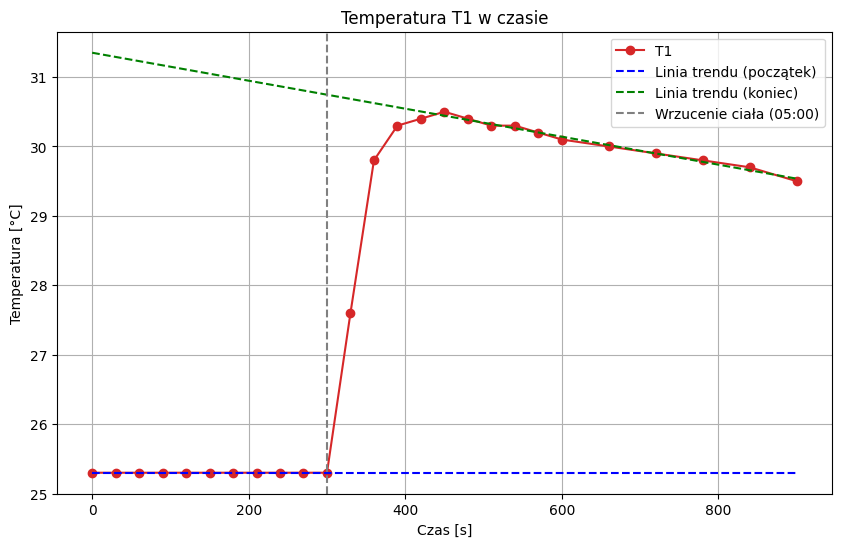
\includegraphics[width=\textwidth]{t1_interpolacja.png}
        \caption{Interpolacja temperatury dla ciała miedzianego}
        \label{fig:t1_interpolacja}
    \end{subfigure}

    \begin{subfigure}[b]{0.65\textwidth}
        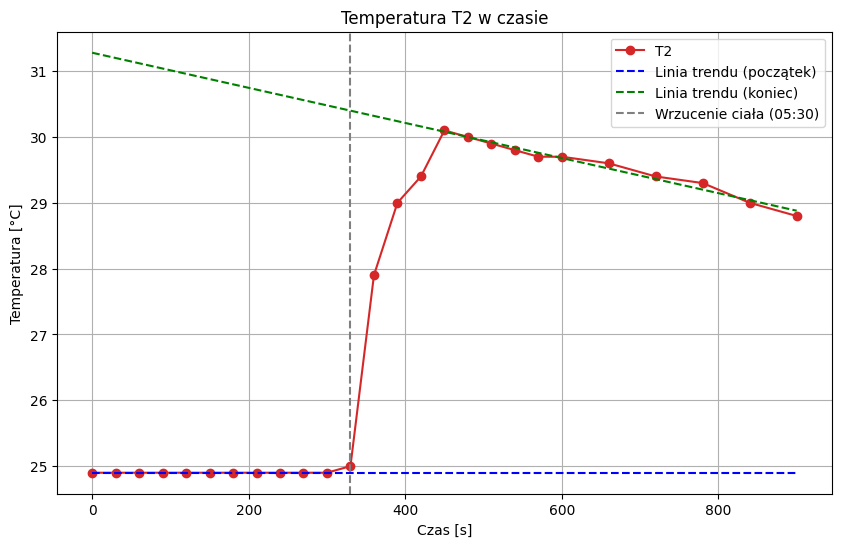
\includegraphics[width=\textwidth]{t2_interpolacja.png}
        \caption{Interpolacja temperatury dla ciała mosiężnego}
        \label{fig:t2_interpolacja}
    \end{subfigure}

    \begin{subfigure}[b]{0.65\textwidth}
        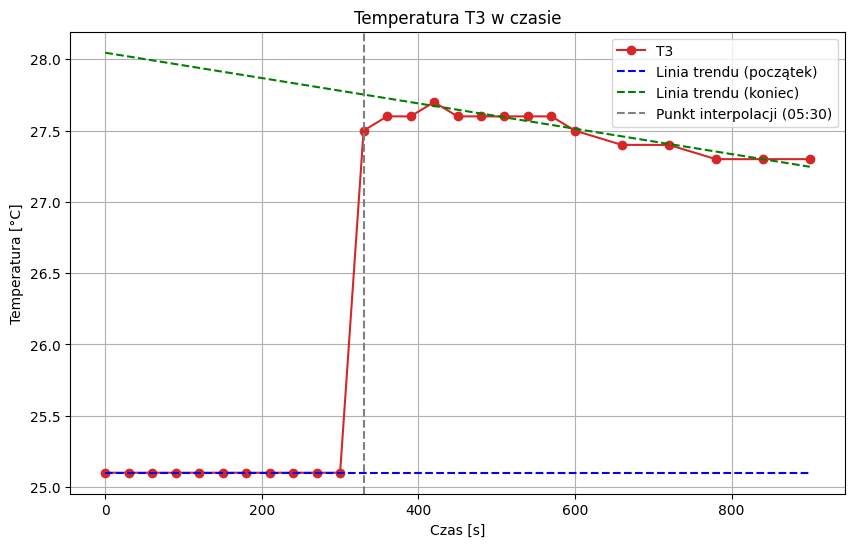
\includegraphics[width=\textwidth]{t3_interpolacja.png}
        \caption{Interpolacja temperatury dla ciała aluminiowego}
        \label{fig:t3_interpolacja}
    \end{subfigure}
    \caption{Wykresy interpolacji temperatury dla badanych ciał}
\end{figure}




\bibliographystyle{plain}
\bibliography{bibliography}

\end{document}
